\documentclass[conference]{IEEEtran}
\IEEEoverridecommandlockouts
% The preceding line is only needed to identify funding in the first footnote. If that is unneeded, please comment it out.
\usepackage{cite}
\usepackage{amsmath,amssymb,amsfonts}
\usepackage{algorithmic}
\usepackage{graphicx}
\usepackage{textcomp}
\usepackage{xcolor}
\usepackage{hyperref}
\usepackage{enumitem}

\usepackage{tabularx,ragged2e,booktabs,caption}

\graphicspath{ {./images/} }
% \renewcommand{\figurename}{Figure}


% \def\fast{Fast~R-CNN}
\newcommand{\fast}[0]{\mbox{Fast~R-CNN}}
\newcommand{\faster}[0]{\mbox{Faster~R-CNN}}

\def\BibTeX{{\rm B\kern-.05em{\sc i\kern-.025em b}\kern-.08em
    T\kern-.1667em\lower.7ex\hbox{E}\kern-.125emX}}
    
\renewcommand{\thetable}{\arabic{table}}
\renewcommand{\tablename}{Table}

\begin{document}

\title{\faster{}: Fast and Unified \\Object Detection System}

\author{\IEEEauthorblockN{Ali Abbasi}
\IEEEauthorblockA{\textit{Department of Computer Engineering} \\
\textit{Sharif University of Technology}\\
Tehran, Iran \\
\href{mailto:a.abbasi@sharif.edu}{a.abbasi@sharif.edu}}
}

\maketitle

\begin{abstract}
This paper proposes methods for improving the speed and accuracy of region-based object detection networks in two steps.
The key idea of both steps is sharing convolutional features of input images for various tasks.
In the first step, special pooling layers called Region of Interest pooling are used on the conv features for extracting features related to that region instead of running the whole CNN separately on each one of them; which results in the primary version of our model, \fast{}.
And in the second step, a CNN-based region proposal method is introduced, which we call 
% Todo
it RPN, that shares input image's conv features with detection network (\fast{}), resulting in the final model, \faster{} network with nearly cost-free region proposals. Doing so, training and testing speed increase drastically while achieving state-of-the-art (or even improving) detection accuracy.
\fast{} trains VGG-16 network 9\texttimes\ times faster than R-CNN and is 213\texttimes\ faster at test time and compared to SPPnet, is 3\texttimes\ and 10\texttimes\ faster in training and testing respectively.
Moreover, our \faster{} model with a very deep network, has a frame rate of $5fps$, including all steps.
\end{abstract}

\begin{IEEEkeywords}
Object Detection, Region Proposal, Region of Interest pooling, Convolutional Neural Networks
\end{IEEEkeywords}

\section{Introduction}
Lately, deep Convolutional Networks (e.g. \cite{a14}) have helped to reach significant and pragmatical results in various computer vision tasks such as image classification \cite{a14} and object detection \cite{a9, a19}. However, because of the more complex nature of object detection 
which arises from the need to localize objects accurately and process a large number of candidates for object locations (proposals), current solutions to this problem (e.g. \cite{a9, a12, a19}) are slow, complicated, and impractical.

The most important drawback of these models is that they
% todo
are designed as a pipeline of multiple stages in which each stage has to be trained separately, making training expensive in time and space.

For solving this problem, we propose a unified training process with a multi-task loss that optimizes different parts of the network simultaneously and therefore results in an effective single-stage network that we call \fast{}.\\
One more important innovation that decreases both training and testing time of the model drastically and is employed in \fast{} is sharing convolution features of the full image across every proposal, 
thanks to Region of Interest (RoI) pooling layers that extract convolution features of proposal region directly from the last layer of Convolutional Network in comparison to R-CNN \cite{a9} which passes every proposal through Convolutional Network.

% with above changes?
\fast{} can train a very deep detection network (VGG-16 \cite{a20}) 9\texttimes\ faster than R-CNN \cite{a9} and 3\texttimes\ faster than SPPnet \cite{a11}. And at runtime, the detection network processes an image in 0.3s (not considering proposal time) while achieving state-of-the-art mAP (mean Average Precision) of 66\% (in comparison to 62\% for R-CNN \cite{a9}).\footnote{All timings are on a Nvidia K40 GPU overclocked to 875 MHz.}

% todo
As explained above, all previously mentioned object detection approaches (including \fast{}) depend on a separate region proposal methods such as Selective Search \cite{b4} which is an order of magnitude slower than our detection network (2 seconds per image), or EdgeBoxes \cite{b6} which consumes as much time as detection step (0.2 seconds per image); which shows computing proposals is a bottleneck in state-of-the-art detection systems in test time.

With the above-mentioned concern in mind, we introduce a
% Todo
new, sophisticated, and effective way of computing proposals, \textit{Region Proposal Networks} (RPNs), which is based on a deep convolutional neural network and can share CNN layers with \fast{} detection network.\\
The RPN is a fully convolutional network and
% todo
is constructed by adding a few additional convolutional
layers that classify "anchor" boxes (candidates for proposal;
% todo!
see Section~\ref{Anchors})
as object or background and regress their region box simultaneously if
% todo: if they are?    
classified as object. By sharing convolutions with the object detector network, computing proposals at test time will become nearly cost-free ($\sim$10ms per image).
For unifying RPN and \fast{} and sharing convolution features, we propose a training process, \textit{Alternating training}, that alternates between fine-tuning for the region proposal task and then fine-tuning for the object detection while keeping the proposals fixed and repeating these steps until convergence. The final model (\faster{}) still has a frame rate of 5fps (including the proposal step too) with very deep models of \cite{a20}.

% todo?
% \section{Related Work}

\section{\faster{}}
Our object detection method, \faster{}, is composed of two modules; a fully convolutional network proposing regions, RPN, and a deep convolutional object detector, \fast{} that uses proposed regions. Therefore RPN can be considered as "attention" \cite{b31} of this system.
The entire system is unified,
% todo: comma?
with convolutional layers shared (Fig.~\ref{FasterRCNN}).
% todo: we will talk about unification in ... ?

\begin{figure}[t]
\centerline{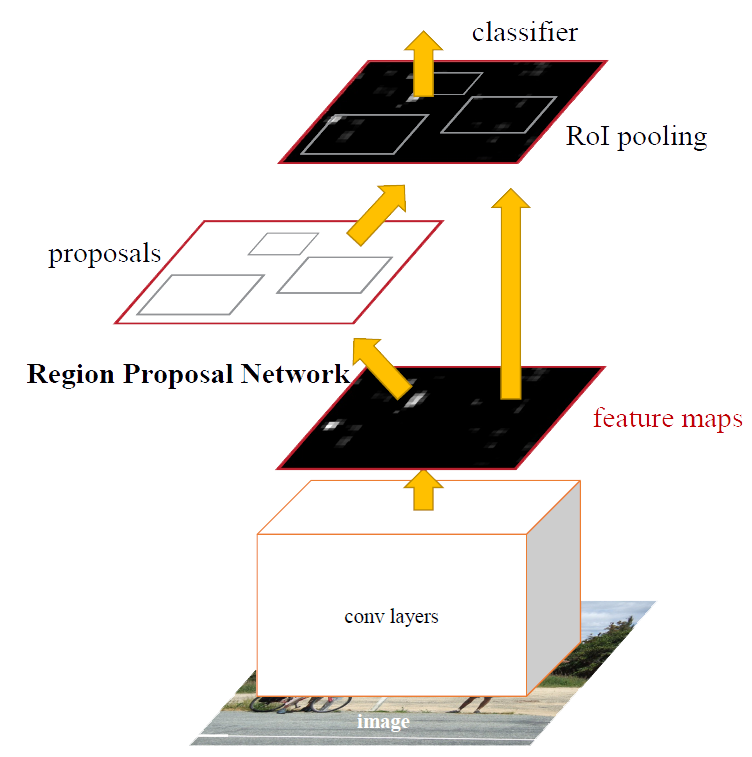
\includegraphics[width=\linewidth]{FasterRCNN.png}}
\caption{\faster{} is a unified combination of RPN and \fast{} modules. RPN module serves as the "attention" of this network.}
\label{FasterRCNN}
\end{figure}

\subsection{\fast{}}
\fast{} module takes as input an image and a series of region proposals. First, the network processes the entire image with a sequence of conv and max pooling layers resulting in a conv feature map of the input image. Then for each proposed region, an RoI pooling layer extracts a feature map of fixed size from conv features and feeds it to a series of fully connected layers. And finally, the output of fully connected layers is fed to two output layers; one that produces softmax probabilities of the region belonging to K classes of objects or the "background" class and another layer that regresses four real-valued numbers of final bounding-box positions for this region if it belongs to one of K object classes.
Fig.~\ref{FastRCNN} illustrates the architecture of Fast R-CNN.

\subsubsection{RoI Pooling Layers}
Each RoI is specified with a tuple of four numbers $(r, c, h, w)$ whose first two numbers, $(r, c)$, determine the top-left corner of the region and $(h, w)$ indicate its height and width. RoI pooling layer, max pools each proposed region to a feature map with a fixed size of $H\times W$ where $H$ and $W$ are hyper-parameters of the model (e.g. $7\times 7$ for VGG-16 in this paper).

RoI pooling works by dividing the $h\times w$ window of the proposed region to  $H\times W$ sub-windows of an approximate size of $\frac{h}{H}\times \frac{w}{W}$ and returning the maximum value in each sub-window 
% todo: that/as
in the same way as a max pooling layer.

\subsubsection{Initializing from Pre-Trained Networks and Fine-Tuning}
\label{InitNetwork}
We use a pre-trained ImageNet \cite{a4} (e.g. VGG-16 \cite{a20}) with some modifications as our network for \fast{}. first, the last max-pooling layer is replaced by an RoI pooling layer with its hyper-parameters set to values compatible with the fully connected layers (e.g. $H=W=7$ for VGG-16). Then, the last fully connected layer and softmax layer which were trained for the 1000-category classification of ImageNet, are replaced with sibling output layers mentioned earlier;
% todo: how to use i.e.
i.e., K+1 class softmax and bounding-box regressor.

% todo: the?
The main benefit of using pre-trained networks is that we can \textit{freeze} parameters of the first layers of the network during training. Because the first layers of neural networks are generic and task-independent \cite{a14} (e.g. distinguishing edges). And for small networks, you can even freeze the entire convolution layers, fine-tuning only fully connected layers. But such is not the case in very deep networks like VGG-16. In our context, fine-tuning VGG-16 as the network used to initialize \fast{}, we realized that it is only necessary to update 9 layers out of 13 conv layers, which speeds up training and saves considerable
% todo: amount of?
GPU memory. Fine-tuning one more conv layer results in $1.3\times$ training time and an almost neglectable increase in mAP, $+0.3\%$.

% todo?
% \subsubsection{Mini-batch Sampling}

\begin{figure}[t]
\centerline{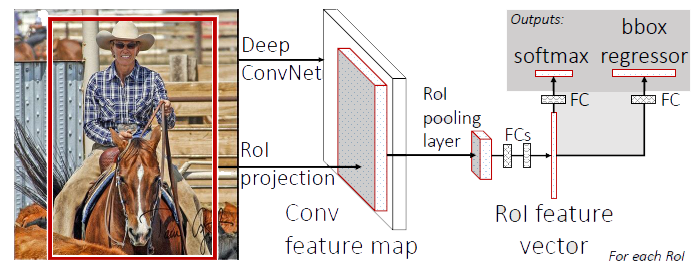
\includegraphics[width=\linewidth]{FastRCNN.png}}
\caption{\fast{} architecture. An input image and a series of regions of interest (RoIs) are given as input into a fully convolutional network. Each RoI is pooled into a fixed-size feature map which is fed to a sequence of fully connected (fc) layers. The network generates two output vectors from fc layers' features per RoI: softmax probabilities and bounding-box regression positions.}
\label{FastRCNN}
\end{figure}
\subsubsection{Multi-task Loss}
As described, network has two sibling outputs for each RoI. The first one is softmax probability distribution over $K+1$ classes, $p = (p_0, \ldots, p_K)$; assigning index $0$ to background class by convention. And the second output is bounding-box's top-left corner positions and box's width and height, $t^k=(t^k_x, t^k_y, t^k_w, t^k_h)$ for $k\in \{1, \ldots, K\}$ \cite{a9}.

In training, each RoI is labeled with a ground-truth class category and bounding box, $u$ and $v$ respectively. We use multi-task loss $L$ in Eq.~\eqref{multTaskLoss} on each RoI to train classification and bounding-box regression simultaneously:
\begin{equation}
\label{multTaskLoss}
L(p, u, t^u, v) = L_{cls}(p, u) + \lambda\left[u\geq 1\right]L_{loc}(t^u, v),
\end{equation}

in which $L_{cls}(p, u) = - \log p_u$ is log loss, a common loss function for classification tasks and $L_{loc}$ is defined over $v$ (ground-truth) and $t^u$ (predicted) tuples for bounding-box.
% todo: sth instead of an?
And $\left[u\geq 1\right]$ is an indicator function omitting $L_{loc}$ from loss term for background proposals.

For bounding-box regression loss, $L_{loc}$ is defined as
\begin{equation}
L_{loc}(t^u, v) = \sum_{i\in \{x, y, w, h\}} \textup{smooth}_{L_1}(t^u_i-v_i),
\label{regLoss}
\end{equation}
in which
\begin{equation}
\textup{smooth}_{L_1}(x)=\left\{ 
\begin{array}{lr}
0.5x^2 & \textup{if $|x| < 1$}\\
|x| - 0.5 & \textup{otherwise}.
\end{array}
\right.
\end{equation}

The hyper-parameter $\lambda$ in Eq.~\eqref{multTaskLoss} balances the effect of two losses. In all of our experiments, $\lambda = 1$.

\subsection{Region Proposal Networks}
A Region Proposal Network (RPN) as input and outputs a set of rectangular object proposals with an objectness score for each, e.i. probability of belonging to one of object classes vs. background.
In our implementation, RPN is going to share computation of convolutional features with a \fast{} object detector.

We use a small $n\times n$ convolution layer followed by a ReLU~\cite{b33} over the shared convolutional layer to map conv features to a lower-dimensional feature vector (512-d for VGG with $n=3$). This feature vector is given as input to two sibling fully connected layers; a box-regressor (\textit{reg}) and a box-classification layer (\textit{cls}).

\subsubsection{Anchors}
\label{Anchors}
The $n\times n$ convolution layer can be seen as a sliding window over the conv feature map. And at each location, we predict $k$ region proposals simultaneously. Therefore \textit{reg} has $4k$ outputs for the coordinates of $k$ boxes and the \textit{cls} has $2k$ outputs, estimating the probability of being an object or background for each of $k$ proposal.

The $k$ proposed outputs of the \textit{reg} layer are parameterized relative to $k$ reference boxes, which we call \textit{anchors}. An anchor is centered at each position of the mentioned sliding window and is associated with three different scales (128, 256, and 512 pixels) and three different aspect ratios (1:1, 1:2, and 2:1), yielding $k=9$ anchors at each position (Fig.~\ref{AnchorsFig}). Thus a conv feature map of size $W\times H$ (typically $\sim 2400$) has $WHk$ anchors in total.

\subsubsection{Region Proposal Network Loss Function}
For training RPNs, we assign a "positive" or "negative" label to each anchor indicating if that anchor represents an object or not. We label an anchor as positive if one of the following conditions is met:
\begin{enumerate}[label=(\roman*)]
\item the anchor has the highest Intersection over Union (IoU) overlap with a ground-truth box, or
\item the anchor has an IoU overlap higher than $0.7$ with any ground-truth box.
\end{enumerate}
And in the same way, non-positive anchors with IoU overlap lower than $0.3$ with all ground-truth boxes are labeled as negative.
After these two steps, unlabeled (neither positive nor negative) anchors are removed from the training process.

With these definitions, we define our loss function for an image as
\begin{equation}
\begin{split}
L\left(\{(p_i, t_i)\}\right) =\ &\frac{1}{N_{cls}}\sum_i L_{cls}(p_i, p_i^*)\\ &+ \lambda \frac{1}{N_{reg}}\sum_i p_i^* L_{reg}(t_i, t_i^*),
\end{split}
\label{RPNLoss}
\end{equation}
in which $i$ is the index of an anchor in a mini-batch, $p_i$ is RPN's predicted objectness probability of the $i$\textsuperscript{th} anchor, and $p_i^*$ is ground-truth label of objectness, i.e., 1 if anchor is labeled positive and 0 if it is labeled negative.
Similarly, $t_i$ and $t_i^*$ are representing the 4 coordinates of predicted and ground-truth bounding box for anchor $i$.
The classification loss is log loss over two classes of object and not object:
\begin{equation}
L_{cls}(p_i, p_i^*) = -p_i^*\log p_i + (1-p_i^*)\log (1-p_i).
\end{equation}
And regression loss is defined exactly as $L_{loc}$ in Eq.~\eqref{regLoss}.

Classification loss and regression loss are normalized by $N_{cls}$ and $N_{reg}$ respectively and the hyper-parameter $\lambda$ balances their effect.
Throughout this paper, we use the mini-batch size (256) and the number of anchor locations for an image ($\sim2400$) as normalizing factors $N_{cls}$ and $N_{reg}$. And we set $\lambda = 10$ so that classification and regression losses are roughly weighted equally.
% todo: for bounding box parameterization

\begin{figure}[t]
\centerline{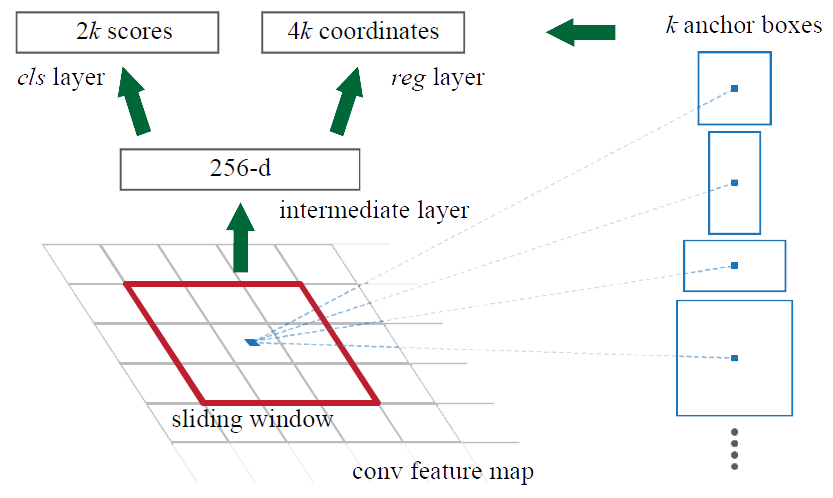
\includegraphics[width=\linewidth]{AnchorsFig.png}}
\caption{A $n\times n$ convolution layer slides over shared conv feature map. And in each position, a vector of features (256-d in VGG) is generated, and k anchor boxes with different
% todo: different As and Bs or different A and Bs?
scales and aspect ratios are proposed; hence \textit{cls} and \textit{reg} layers output $2k$ scores and $4k$ coordinates at each position respectively.}
\label{AnchorsFig}
\end{figure}

\begin{table*}[t]
\caption{\small{Detection results on PASCAL VOC 2007 test set. The detector is \fast{} initialized with VGG-16.\\Training data: "07": VOC 2007 trainval, "07+12": union set of VOC 2007 trainval and VOC 2012 trainval, "C+07+12": union set of VOC 2007, VOC 2012, and MS COCO trainvals.
% For RPN, the train-time number of proposals for \fast{} is 2000.
}}
\begin{minipage}{\linewidth}
\begin{center}
\renewcommand\footnoterule{ \kern -1ex}
% \renewcommand{\thempfootnote}{\fnsymbol{mpfootnote}}
\begin{tabular}{c c|c|c}
method & number of proposals & data & mAP(\%)\\
\hline
\hline
SS & 2000 & 07 & 66.9\\
SS & 2000 & 07+12 & 70.0\\
\hline
RPN+VGG, unshared & 300 & 07 & 68.5\\
RPN+VGG, shared & 300 & 07 & 69.9\\
RPN+VGG, shared & 300 & 07+12 & \textbf{73.2}\\
\hline
RPN+VGG, shared & 300 & C+07+12 & \textbf{78.8}
\end{tabular}
\end{center}
\end{minipage}
\label{VOC2007Result}
\end{table*}

\begin{table*}[t]
\caption{\small{Results on PASCAL VOC 2007 test set with Fast R-CNN detectors and VGG-16. For RPN, the train-time
proposals for Fast R-CNN are 2000. RPN\textsuperscript{*} denotes the unshared feature version.}}
\begin{minipage}{\linewidth}
\begin{center}
\renewcommand\footnoterule{\kern -1ex}
\setlength{\tabcolsep}{2.5pt}
\begin{tabular}{c|c|c|c|ccccccccccccccccccccc}
method  & \# box &  data  & mAP  & \footnotesize{areo}  & \footnotesize{bike}  & \footnotesize{bird} &  \footnotesize{boat} & \footnotesize{bottle} & \footnotesize{bus} & \footnotesize{car} & \footnotesize{cat} & \footnotesize{chair} & \footnotesize{cow} & \footnotesize{table} & \footnotesize{dog} & \footnotesize{horse} & \footnotesize{mbike} & \footnotesize{person}  & \footnotesize{plant} & \footnotesize{sheep} &\footnotesize{sofa} & \footnotesize{train} &  \footnotesize{tv}\\
\hline
\hline
SS & 2000 & 07 & 66.9 & 74.5 & 78.3 & 69.2 & 53.2 & 36.6 & 77.3 & 78.2 & 82.0 & 40.7 & 72.7 & 67.9 & 79.6 & 79.2 & 73.0 & 69.0 & 30.1 & 65.4 & 70.2 & 75.8 & 65.8\\

SS & 2000 & 07+12 & 70.0 & 77.0 & 78.1 & 69.3 & 59.4 & 38.3 & 81.6 & 78.6 & 86.7 & 42.8 & 78.8 & 68.9 & 84.7 & 82.0 & 76.6 & 69.9 & 31.8 & 70.1 & 74.8 & 80.4 & 70.4\\
\hline

RPN\textsuperscript{*} & 300 & 07 & 68.5 & 74.1 & 77.2 & 67.7 & 53.9 & 51.0 & 75.1 & 79.2 & 78.9 & 50.7 & 78.0 & 61.1 & 79.1 & 81.9 & 72.2 & 75.9 & 37.2 & 71.4 & 62.5 & 77.4 & 66.4\\

RPN & 300 & 07 & 69.9 & 70.0 & 80.6 & 70.1 & 57.3 & 49.9 & 78.2 & 80.4 & 82.0 & 52.2 & 75.3 & 67.2 & 80.3 & 79.8 & 75.0 & 76.3 & 39.1 & 68.3 & 67.3 & 81.1 & 67.6\\

RPN & 300 & 07+12 & 73.2 & 76.5 & 79.0 & 70.9 & 65.5 & 52.1 & 83.1 & 84.7 & 86.4 & 52.0 & 81.9 & 65.7 & 84.8 & 84.6 & 77.5 & 76.7 & 38.8 & 73.6 & 73.9 & 83.0 & 72.6\\

RPN & 300 & C+07+12 & \textbf{78.8} & \textbf{84.3} & \textbf{82.0} & \textbf{77.7} & \textbf{68.9} & \textbf{65.7} & \textbf{88.1} &\textbf{ 88.4} & \textbf{88.9} & \textbf{63.6} & \textbf{86.3} & \textbf{70.8} & \textbf{85.9} & \textbf{87.6} & \textbf{80.1} & \textbf{82.3} & \textbf{53.6} & \textbf{80.4} & \textbf{75.8} & \textbf{86.6} & \textbf{78.9}
\end{tabular}
\end{center}
\end{minipage}
\label{ComprehensiveResults}
\end{table*}

\begin{table*}[t]
\caption{\small{Results on PASCAL VOC 2012 test set with Fast R-CNN detectors and VGG-16. For RPN, the train-time
proposals for Fast R-CNN are 2000.\\Training data: "07++12": union set of VOC 2007 trainval+test and VOC 2012 trainval, "C+07++12": union set of VOC 2007 trainval+test and VOC 2012 and MS COCO trainvals.}}
\begin{minipage}{\linewidth}
\begin{center}
\renewcommand\footnoterule{\kern -1ex}
\setlength{\tabcolsep}{2.5pt}
\begin{tabular}{c|c|c|c|ccccccccccccccccccccc}
method  & \# box &  data  & mAP  & \footnotesize{areo}  & \footnotesize{bike}  & \footnotesize{bird} &  \footnotesize{boat} & \footnotesize{bottle} & \footnotesize{bus} & \footnotesize{car} & \footnotesize{cat} & \footnotesize{chair} & \footnotesize{cow} & \footnotesize{table} & \footnotesize{dog} & \footnotesize{horse} & \footnotesize{mbike} & \footnotesize{person}  & \footnotesize{plant} & \footnotesize{sheep} &\footnotesize{sofa} & \footnotesize{train} &  \footnotesize{tv}\\
\hline
\hline
SS & 2000 & 12 & 65.7 & 80.3 & 74.7 & 66.9 & 46.9 & 37.7 & 73.9 & 68.6 & 87.7 & 41.7 & 71.1 & 51.1 & 86.0 & 77.8 & 79.8 & 69.8 & 32.1 & 65.5 & 63.8 & 76.4 & 61.7\\
SS & 2000 & 07++12 & 68.4 & 82.3 & 78.4 & 70.8 & 52.3 & 38.7 & 77.8 & 71.6 & 89.3 & 44.2 & 73.0 & 55.0 & 87.5 & 80.5 & 80.8 & 72.0 & 35.1 & 68.3 & \textbf{65.7} & 80.4 & 64.2\\
\hline
RPN & 300 & 12 & 67.0 & 82.3 & 76.4 & 71.0 & 48.4 & 45.2 & 72.1 & 72.3 & 87.3 & 42.2 & 73.7 & 50.0 & 86.8 & 78.7 & 78.4 & 77.4 & 34.5 & 70.1 & 57.1 & 77.1 & 58.9\\
RPN & 300 & 07++12 & 70.4 & 84.9 & 79.8 & 74.3 & 53.9 & 49.8 & 77.5 & 75.9 & 88.5 & 45.6 & 77.1 & 55.3 & 86.9 & 81.7 & 80.9 & 79.6 & 40.1 & 72.6 & 60.9 & 81.2 & 61.5\\
RPN & 300 & C+07++12 &  \textbf{75.9} &  \textbf{87.4} &  \textbf{83.6} &  \textbf{76.8} &  \textbf{62.9} &  \textbf{59.6} &  \textbf{81.9} &  \textbf{82.0} &  \textbf{91.3} &  \textbf{54.9} &  \textbf{82.6} &  \textbf{59.0} &  \textbf{89.0} &  \textbf{85.5} &  \textbf{84.7} &  \textbf{84.1} &  \textbf{52.2} &  \textbf{78.9} &  65.5 &  \textbf{85.4} &  \textbf{70.2}
\end{tabular}
\end{center}
\end{minipage}
\label{ComprehensiveResults2012}
\end{table*}

\subsubsection{Non-Maximum Suppression}
Some of the object proposals proposed by RPN may have high overlaps with each other and may cause our detection network to process one image multiple times, decreasing training and testing speed. Non-maximum suppression (NMS) based on proposed regions' \textit{cls} scores is used to deal with this redundancy and make the proposal network more efficient. IoU threshold for NMS is fixed at 0.7, which will leave us about 2000 proposals per image. After NMs, top-$N$ ranked proposals based on their \textit{cls} score are used for detection. Throughout this paper, \fast{} is trained using 2000 RPN proposals but is evaluated with different number of proposals at test time (we will show in test time, that using top 300 proposals is sufficient).


\subsection{Sharing Features for RPN and \fast{}}
So far training process of \fast{} and RPN modules have been described independently. Now we describe methods for training a unified network composed of these two modules with shared convolutional features.

Training RPN and \fast{} independently will update parameters of convolutional layers differently and naive sharing CNN layers of one of the modules after they have been trained independently is not a solution to our purpose. Therefore, we use a technique called \textit{alternative training}. In this technique, first, the RPN is trained and its proposals are used to train \fast{} independently with both networks initialized with an ImageNet pre-trained model and fine-tuned as described in Section~\ref{InitNetwork}. Next, CNN layers of \fast{} are used to initialize the RPN network. With shared convolutional layers frozen, layers that are unique to RPN are fine-tuned. At this point the two networks share convolutional layers. And in the final step, again with shared convolutional layers frozen, we fine-tune unique layers of \fast{}. This process of alternative training could be run for more iterations, but we have observed trivial improvements.

\begin{table*}[t]
\caption{\small{\textbf{Timings} (ms) on a K40 GPU, except Selective Search (SS) proposals which are evaluated on a CPU. "Region-wise" includes NMS, pooling, fully-connected, and softmax layers.}}
\begin{minipage}{\linewidth}
\begin{center}
\renewcommand\footnoterule{ \kern -1ex}
\begin{tabular}{c|c|ccc|c|c}
model & system & conv &  \# proposal & region-wise & total & rate\\
\hline
\hline
VGG  & SS + Fast R-CNN &  146 &  1510 &  174 &  1830 &  0.5 fps\\
VGG &  RPN + Fast R-CNN &  141  & \textbf{10} &  47 &  \textbf{198}  & \textbf{5 fps}
\end{tabular}
\end{center}
\end{minipage}
\label{Timing}
\end{table*}

\section{Experimental Results}
% todo: contributions
We mainly evaluate our model on the PASCAL VOC 2007 detection benchmark \cite{b11} and also the union of it with other datasets such as PASCAL VOC 2012 and Microsoft COCO object detection dataset \cite{b12}. A good object detector network should improve when supplied with more training data. Zhu \textit{et al.} \cite{a24} showed that DPM \cite{a8} mAP saturates after only a few hundred to thousand training images. This aspect of our model will be discussed shortly. VOC 2007 dataset consists of about $5k$ trainval images and $5k$ test images over 20 object classes. We evaluate our model with the mean Average Precision (mAP) metric which is the actual metric for object detection and object proposal proxy metrics for RPN are not considered in this paper.

Table~\ref{VOC2007Result} shows the results of using the VGG-16 network for both proposal and detection purposes. Using RPN+VGG (RPN network initialized with VGG), the result is $68.5\%$ for \textit{unshared} features, slightly higher than the SS baseline. Which is the result of actively trained networks in RPN instead of pre-defined methods in Selective Search. For the feature-\textit{shared} version, the result is $69.9\%$, better than the strong Selective Search baseline and \textit{unshared} features variant and yet, with nearly cost-free proposals.
Further training the model on the union set of PASCAL VOC 2007 trainval and 2012 trainval results in an mAP of $\mathbf{73.2\%}$. And similarly training \faster{} on the union set of PASCAL VOC 2007 trainval, 2012 trainval, and MS COCO trainval, results in an mAP of $\mathbf{78.8\%}$, proving our claim about \faster{} improving when supplied with more training data. Table~\ref{ComprehensiveResults} and Table~\ref{ComprehensiveResults2012} show the detailed numbers and the model's mAP for each object class.

The running time of the entire object detection system is summarized in Table~\ref{Timing}. Depending on the input image, Selective Search can take between 1 to 2 seconds, and its average value is used here. 
\faster{} with VGG-16 takes near real-time $\mathbf{198ms}$ in total for both proposal and detection, with the RPN only taking $10ms$ computing its unique layers. Our region-wise computation is also faster, because of fewer proposals (300 per image vs. 2000 per image).

Fig.~\ref{FasterRCNN-VOC2007} illustrates samples of \faster{} network performance on the PASCAL VOC 2007 test set.

\begin{figure}[t]
\centerline{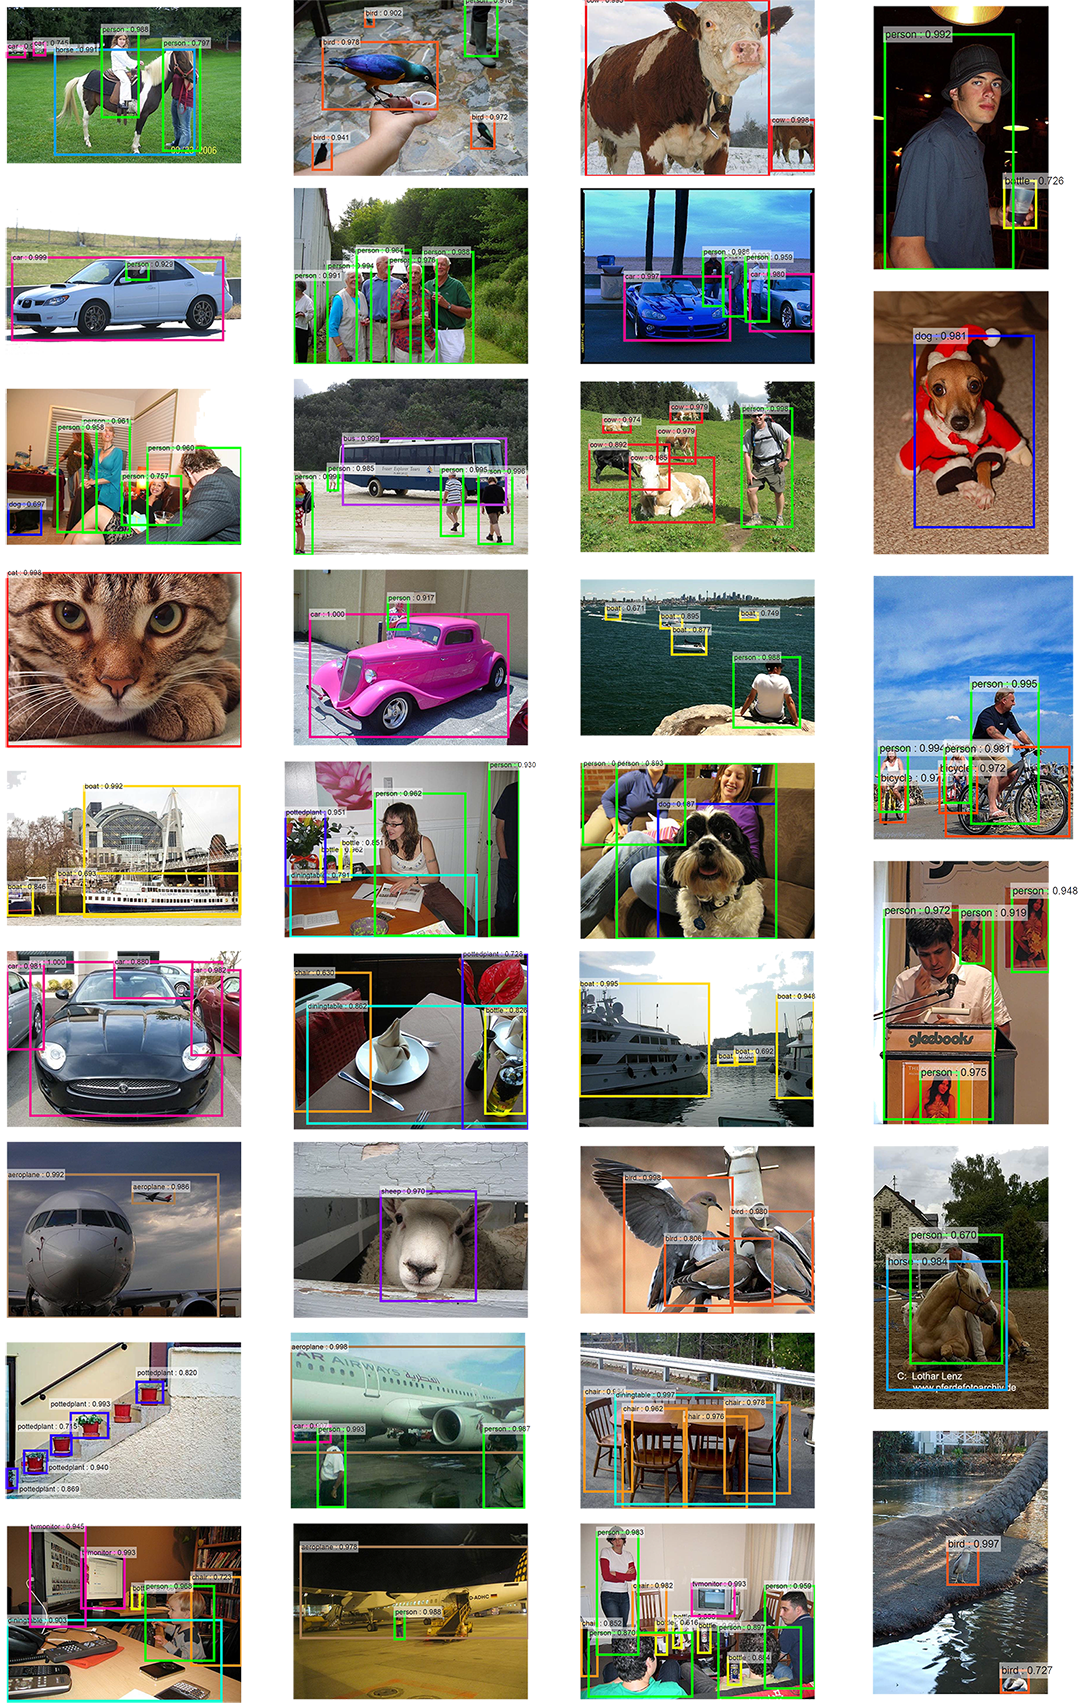
\includegraphics[width=\linewidth]{images/FasterRCNN-VOC07-compressed.png}}
\caption{Selected examples of \faster{} network's object detection results on the PASCAL VOC 2007 test set. The model is initialized with VGG-16 and the training data is PASCAL VOC 07+12 trainval (achieving 73.2\% mAP on the 2007 test set). Our model detects objects with various scales and aspect ratios. Each output box is associated with a category label and a softmax score in the range $[0, 1]$. Displayed objects have a score greater than 0.6. The running time for obtaining these results is \textbf{198ms} per image, including all steps.}
\label{FasterRCNN-VOC2007}
\end{figure}

\section{Conclusion}
This paper proposes a clean and fast way of training object detector networks, along with an efficient, accurate, and yet nearly cost-free region proposal generation by sharing convolution features across two modules. Our method enables a very deep neural network object detection system to run at near-real-time frame rates while achieving state-of-the-art detection accuracy metrics and improves previous results due to improved region proposal quality.

% \section*{Acknowledgment}

% \section*{References}
\begin{thebibliography}{00}

% b3
\bibitem{a20} K. Simonyan, A. Zisserman, "Very deep convolutional networks for large-scale image recognition," in \textit{International Conference on Learning Representations (ICLR)}, 2015.

\bibitem{a9} R. Girshick, J. Donahue, T. Darrell, and J. Malik, "Rich feature hierarchies for accurate object detection and semantic segmentation," in \textit{Conference on Computer Vision and Pattern Recognition (CVPR)}, 2014.

\bibitem{a4} J. Deng, W. Dong, R. Socher, L.-J. Li, K. Li, and L. Fei-Fei, "ImageNet: A large-scale hierarchical image database," in \textit{Conference on Computer Vision and Pattern Recognition (CVPR)}, 2009.

\bibitem{b4} J. R. Uijlings, K. E. van de Sande, T. Gevers, and A. W. Smeulders, "Selective search for object recognition," in \textit{International Journal of Computer Vision (IJCV)}, 2013.

\bibitem{b6} C. L. Zitnick and P. Doll´ar, "Edge boxes: Locating object proposals from edges," in \textit{European Conference on Computer Vision (ECCV)}, 2014.

\bibitem{b11} M. Everingham, L. Van Gool, C. K. I. Williams, J. Winn, and A. Zisserman, "The PASCAL Visual Object Classes Challenge 2007 (VOC2007) Results," 2007.

\bibitem{a11} K. He, X. Zhang, S. Ren, and J. Sun, "Spatial pyramid pooling in deep convolutional networks for visual recognition," in \textit{European Conference on Computer Vision (ECCV)}, 2014.

\bibitem{a12} J. H. Hosang, R. Benenson, P. Doll´ar, and B. Schiele, "What makes for effective detection proposals?," \textit{arXiv preprint arXiv:1502.05082}, 2015.

\bibitem{a14} A. Krizhevsky, I. Sutskever, and G. Hinton, "ImageNet classification with deep convolutional neural networks," in \textit{Neural Information Processing Systems (NIPS)}, 2012.

\bibitem{a19} P. Sermanet, D. Eigen, X. Zhang, M. Mathieu, R. Fergus, and Y. LeCun, "OverFeat: Integrated Recognition, Localization and Detection using Convolutional Networks," in \textit{International Conference on Learning Representations (ICLR)}, 2014.

\bibitem{b12} T.-Y. Lin, M. Maire, S. Belongie, J. Hays, P. Perona, D. Ramanan, P. Doll´ar, and C. L. Zitnick, "Microsoft COCO: Common Objects in Context," in \textit{European Conference on Computer Vision (ECCV)}, 2014.

\bibitem{a8} P. Felzenszwalb, R. Girshick, D. McAllester, and D. Ramanan, "Object detection with discriminatively trained part based models," \textit{IEEE Transactions on Pattern Analysis and Machine Intelligence (TPAMI)}, 2010.

\bibitem{b33} V. Nair and G. E. Hinton, "Rectified linear units improve restricted Boltzmann machines," in \textit{International Conference on Machine Learning (ICML)}, 2010.

\bibitem{a24} X. Zhu, C. Vondrick, D. Ramanan, and C. Fowlkes, "Do we need more training data or better models for object detection?," in \textit{British Machine Vision Conference (BMVC)}, 2012.

\bibitem{b31} J. K. Chorowski, D. Bahdanau, D. Serdyuk, K. Cho, and
Y. Bengio, “Attention-based models for speech recognition,” in
\textit{Neural Information Processing Systems (NIPS)}, 2015.

\end{thebibliography}
\end{document}
